\documentclass[10pt]{article}
\usepackage[usenames]{color} %used for font color
\usepackage{amssymb} %maths
\usepackage{amsmath} %maths
\usepackage{url} %maths
\usepackage[utf8]{inputenc} %useful to type directly diacritic characters
\usepackage{fancyhdr}
\usepackage{graphicx}
% customize fancyhdr package
\pagestyle{fancy} \fancyhf{}
\lhead{
\includegraphics[width=1.5cm]{uni-logo.png}
 \hspace*{.2ex}\parbox[b]{.85\textwidth}{\footnotesize
\hfill   Exercises Week 49/50 in DM561, 2021, IMADA, SDU}}
\rfoot{Page \thepage}

\begin{document}
\noindent {\bf Exercise 1: PCA Visually}\\
Consider 100 students with Physics and Statistics grades shown in the two diagram below. 

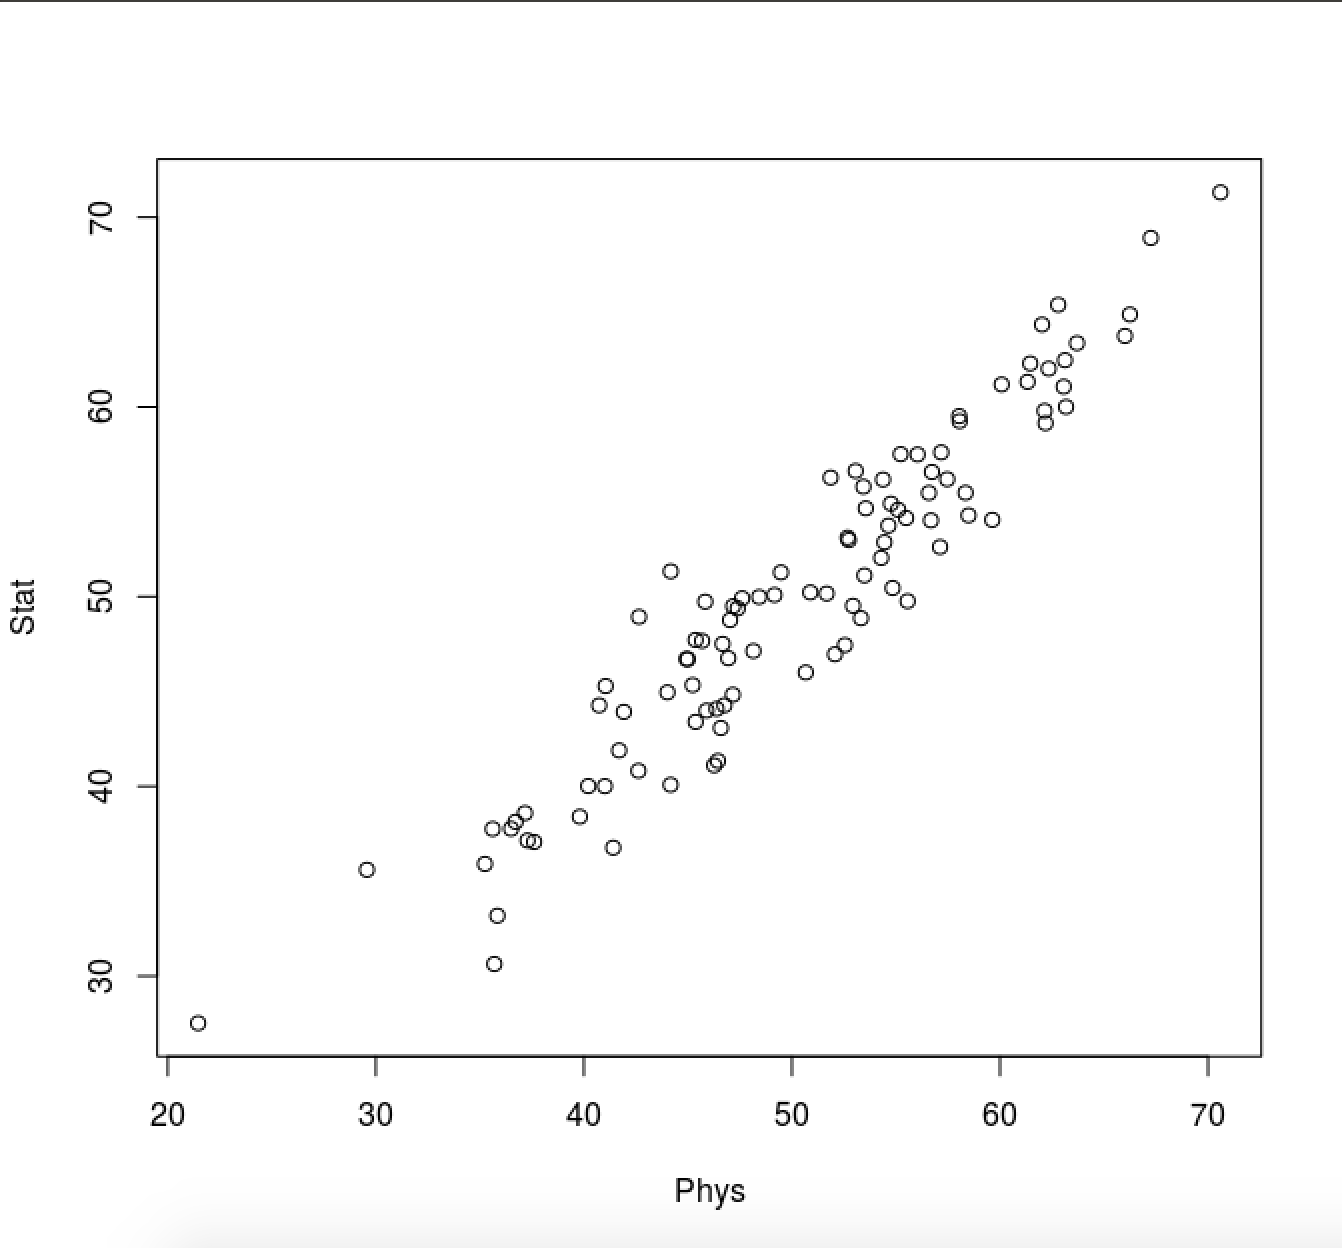
\includegraphics[width=6cm]{1.png}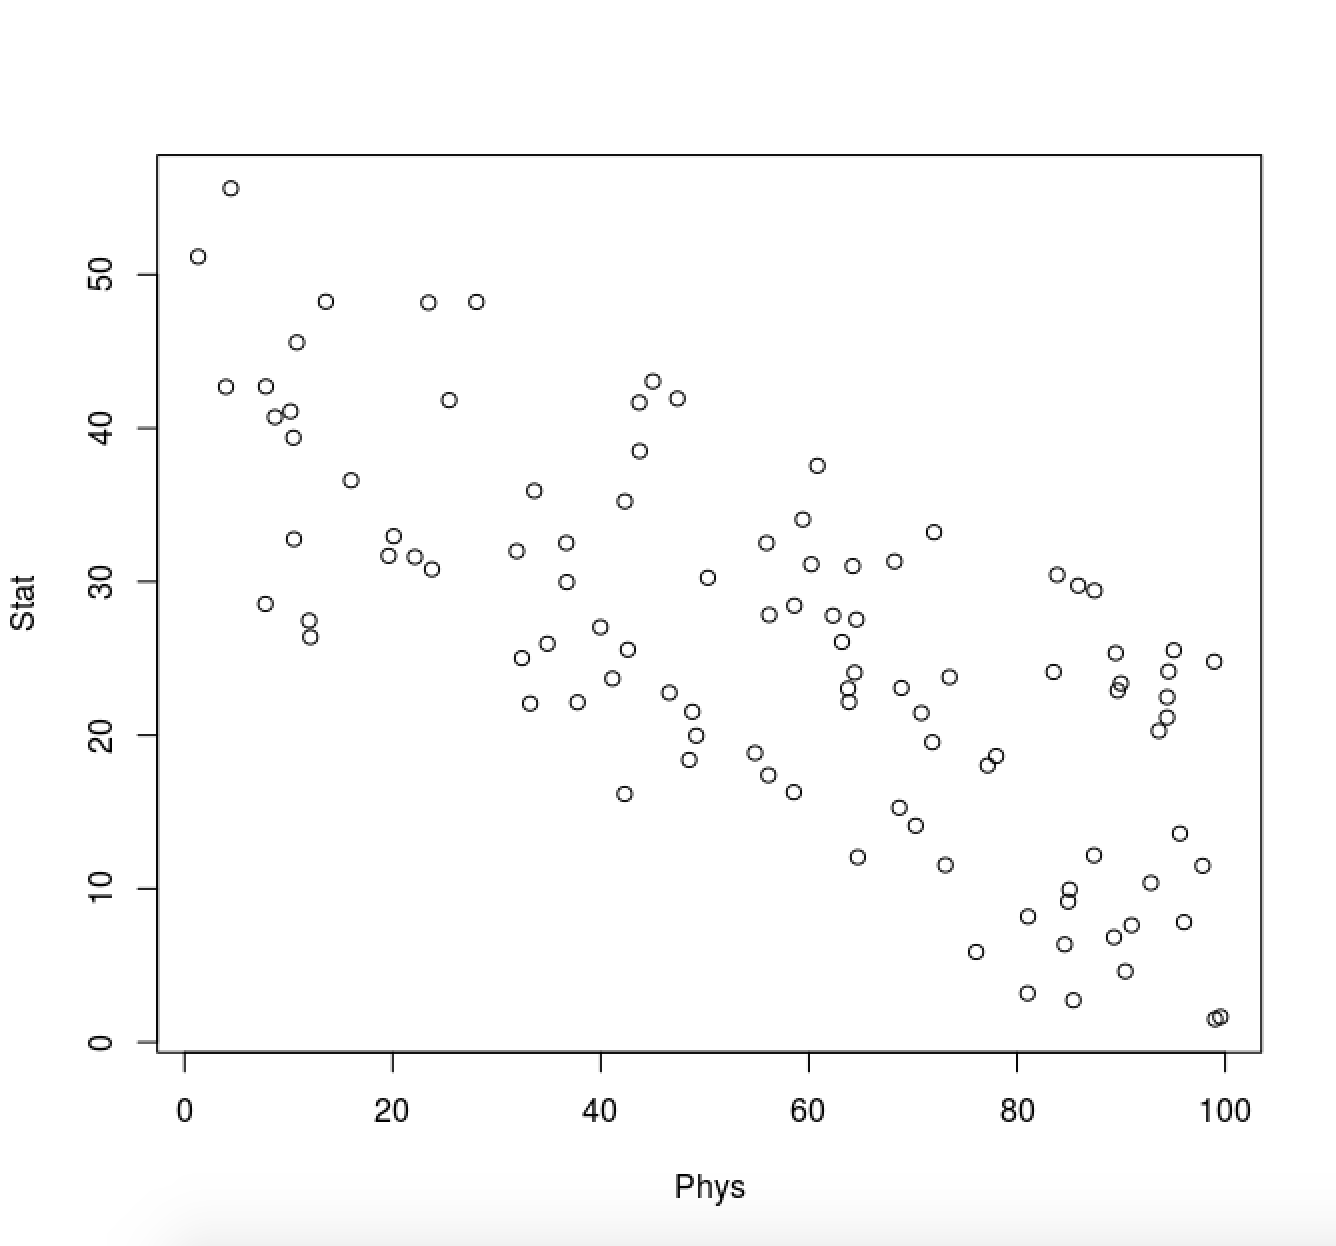
\includegraphics[width=6cm]{2.png}

For each of the diagrams:
\begin{enumerate}
\item Which is the direction (as a vector) along which the data varies the most?
\item What is (roughly) the point representing the mean value of the statistics/mathematics degree?
\end{enumerate}


\noindent {\bf Exercise 2: Covariance Matrix}\\
% see https://stattrek.com/matrix-algebra/covariance-matrix.aspx#Problem1 
Assume the following grades:

\begin{center}
\begin{tabular}{rrrr}
Student & Math & English & Art\\
\hline
1 & 90 & 60 & 90\\
2 & 90 & 90 & 30\\
3 & 60 & 60 & 60\\
4 & 60 & 60 & 90\\
5 & 30 & 30 & 30\\
\hline
\end{tabular}
\end{center}

\begin{enumerate}
\item Define a matrix $X'$ where the rows represent samples (students), and the columns represent features (the different tests).
\item Perform mean centering: subtract each data value from its variable's measured mean so that its empirical mean (average) is zero, call the resulting matrix $X$. 
\item Without computing, what do you expect the covariance between a) Math and English and b) English and Art to be? Postive or negative?
\item Ignoring Bessel's correction, which formula (cmp. slide 9) should be used to compute the covariance matrix?
\item Compute the variance of each test grades and the covariance between the test grades.
\item Determine the covariance matrix a) with Bessel's corection, b) without Bessel's correction.
\end{enumerate}

\noindent {\bf Exercise 3: Projection onto new feature space}\\
When analysing the Iris dataset, we stored the data in form of a $150 \times 4$ matrix where the columns are the different features, and every row represents a separate flower sample. Let's call this matrix $X$. Given the first and the second principal component $w_1$ and $w_2$.
\begin{enumerate}
\item How do we, using matrix multiplication, project the 4-dimensional feature space onto a new 2-dimensional feature space that is spanned by $w_1$ and $w_2$? How does this relate to the formula on page 7 of the slide set?
\item Give the sizes of the matrices that you used in 1.)
\end{enumerate}

\noindent {\bf Exercise 4: Eigenfaces}\\
In your last mandatory assignment you will be using the PCA
functionality from OpenCV (\url{https://opencv.org/}). For this
exercise, we will use another set of tools, namely Google's Colabatory
framework \url{https://colab.research.google.com} and,
\texttt{scikit-learn} (\url{https://scikit-learn.org}), a free
software machine learning library for Python for data analytics,
statistics, machine learning, and \texttt{Scipy}
(\url{https://www.scipy.org/}, the scientific Python ecosystem). All
of those in itself can be quite overwhelming, however, the idea of
this exercise is to show you how easy it is to use and integrate all
those.

Proceed as follows:
\begin{enumerate}
\item Download the Jupyter notebook \texttt{plot\_eigenfaces.ipynb} from here : \url{https://www.scipy-lectures.org/packages/scikit-learn/auto_examples/plot_eigenfaces.html} (at the very end of the page).
\item Upload the notebook to \url{https://colab.research.google.com}.
\item Run the cells subsequently (you can safely ignore everything related to Support Vector classification, and anything after ``Doing the Learning: Support Vector Machines'').
  \item Add a cell (after cell 8) and print the vector in the 150-dimensional Eigenface-space that corresponds to the projection of the first image in the test dataset \texttt{X\_test}.
\end{enumerate}
\end{document}
%%% Local Variables:
%%% mode: latex
%%% TeX-master: t
%%% End:
